% Options for packages loaded elsewhere
\PassOptionsToPackage{unicode}{hyperref}
\PassOptionsToPackage{hyphens}{url}
\PassOptionsToPackage{dvipsnames,svgnames*,x11names*}{xcolor}
%
\documentclass[
  11pt,
]{article}
\usepackage{lmodern}
\usepackage{setspace}
\usepackage{amssymb,amsmath}
\usepackage{ifxetex,ifluatex}
\ifnum 0\ifxetex 1\fi\ifluatex 1\fi=0 % if pdftex
  \usepackage[T1]{fontenc}
  \usepackage[utf8]{inputenc}
  \usepackage{textcomp} % provide euro and other symbols
\else % if luatex or xetex
  \usepackage{unicode-math}
  \defaultfontfeatures{Scale=MatchLowercase}
  \defaultfontfeatures[\rmfamily]{Ligatures=TeX,Scale=1}
  \setmainfont[]{Times New Roman}
  \setsansfont[]{Times New Roman}
\fi
% Use upquote if available, for straight quotes in verbatim environments
\IfFileExists{upquote.sty}{\usepackage{upquote}}{}
\IfFileExists{microtype.sty}{% use microtype if available
  \usepackage[]{microtype}
  \UseMicrotypeSet[protrusion]{basicmath} % disable protrusion for tt fonts
}{}
\makeatletter
\@ifundefined{KOMAClassName}{% if non-KOMA class
  \IfFileExists{parskip.sty}{%
    \usepackage{parskip}
  }{% else
    \setlength{\parindent}{0pt}
    \setlength{\parskip}{6pt plus 2pt minus 1pt}}
}{% if KOMA class
  \KOMAoptions{parskip=half}}
\makeatother
\usepackage{xcolor}
\IfFileExists{xurl.sty}{\usepackage{xurl}}{} % add URL line breaks if available
\IfFileExists{bookmark.sty}{\usepackage{bookmark}}{\usepackage{hyperref}}
\hypersetup{
  colorlinks=true,
  linkcolor=Maroon,
  filecolor=Maroon,
  citecolor=Blue,
  urlcolor=Blue,
  pdfcreator={LaTeX via pandoc}}
\urlstyle{same} % disable monospaced font for URLs
\usepackage[margin=1in]{geometry}
\usepackage{longtable,booktabs}
% Correct order of tables after \paragraph or \subparagraph
\usepackage{etoolbox}
\makeatletter
\patchcmd\longtable{\par}{\if@noskipsec\mbox{}\fi\par}{}{}
\makeatother
% Allow footnotes in longtable head/foot
\IfFileExists{footnotehyper.sty}{\usepackage{footnotehyper}}{\usepackage{footnote}}
\makesavenoteenv{longtable}
\usepackage{graphicx,grffile}
\makeatletter
\def\maxwidth{\ifdim\Gin@nat@width>\linewidth\linewidth\else\Gin@nat@width\fi}
\def\maxheight{\ifdim\Gin@nat@height>\textheight\textheight\else\Gin@nat@height\fi}
\makeatother
% Scale images if necessary, so that they will not overflow the page
% margins by default, and it is still possible to overwrite the defaults
% using explicit options in \includegraphics[width, height, ...]{}
\setkeys{Gin}{width=\maxwidth,height=\maxheight,keepaspectratio}
% Set default figure placement to htbp
\makeatletter
\def\fps@figure{htbp}
\makeatother
\setlength{\emergencystretch}{3em} % prevent overfull lines
\providecommand{\tightlist}{%
  \setlength{\itemsep}{0pt}\setlength{\parskip}{0pt}}
\setcounter{secnumdepth}{5}
\usepackage{mathtools}

\title{\vspace{1cm}Does Spending Time with Your Child Decreases Your Income?\vspace{0.5cm}\\}
\usepackage{etoolbox}
\makeatletter
\providecommand{\subtitle}[1]{% add subtitle to \maketitle
  \apptocmd{\@title}{\par {\large #1 \par}}{}{}
}
\makeatother
\subtitle{An Investigation on the Causal Effect of Parental Leave on Income in Germany \vspace{0.5cm}}
\author{Sophie Hensgen\\
University of Mannheim\\
Matricle number: 1560750}
\date{2021-03-16\\}

\begin{document}
\maketitle

\setstretch{1.2}
\hypertarget{introduction}{%
\section{Introduction}\label{introduction}}

In the past 5 years (2015 - 2019) the number of persons which received parental allowance in Germany increased about almost 20 \% from 1,561,597 to 1,865,129. The proportion of men who have benefited from it increased by 3.5\% and now accounts for almost a quarter of those receiving parental benefits. Although there is a continuing trend for more men to take parental leave (PL), there is still a high gender wage gap. Women stay longer in parental leave, in fact on average four times as long as men (Statistisches Bundesamt \protect\hyperlink{ref-statistisches_bundesamt_zeitreihe_2020}{2020}).

Many researchers have addressed this issue to find out whether parental leave could possibly be responsible for the gender wage gap.

However, no clear results have been found yet.
There is evidence that there is an effect of parental leave on income. That said, scholars are indecisive on why this is the case. Some argue, that the time spend in parental leave could lead to decreasing someones knowledge and skill level (Evertsson \protect\hyperlink{ref-evertsson_parental_2016}{2016}). Especially compared to someone which had the same level to begin with. Thus, if they try to re-enter the workforce, they would have to start at a lower position or would be at a disadvantage in terms of promotions due to the missed practice (Gabriele Mari and Cutuli \protect\hyperlink{ref-gabriele_mari_parental_2019}{2019}; Hofferth and Curtin \protect\hyperlink{ref-hofferth_parental_2006}{2006}). This theory is also known as the human capital theory. On the other hand, scholars present another explanation, the signal theory(Albrecht et al. \protect\hyperlink{ref-albrecht_career_1999}{1999}; Evertsson \protect\hyperlink{ref-evertsson_parental_2016}{2016}).
Not only should it explain the difference between persons who been on parental leave and the ones that weren't, but also the differences between genders. As the human capital theory should have the same consequences despite the gender (Evertsson \protect\hyperlink{ref-evertsson_parental_2016}{2016}), the signalling theory tries to explain why there is difference. In principle, the use of parental leave could be seen as less committed to the company. Thus, when it comes to promotions, employers might prefer someone who was not on parental leave to someone who was on parental leave. So some scholar claim, that this signal might be harder on men (Albrecht et al. \protect\hyperlink{ref-albrecht_career_1999}{1999}; Evertsson \protect\hyperlink{ref-evertsson_parental_2016}{2016}; Stafford and Sundström \protect\hyperlink{ref-stafford_time_1996}{1996}), but at the same time other argue that it is more harmful to women (Ridgeway and Correll \protect\hyperlink{ref-ridgeway_unpacking_2004}{2004}). I will go into this in more detail later.

** Parts excluded due to Word Limit **

All in all, there is the possibility that the effect of human capital and signal theory might diminish over time. After many years, it might not matter if you missed a year, other aspects might become more important. Alternatively, it could be that one has gained such disadvantages from the parental leave that these could have far-reaching consequences. If the former is true, this could lead to more men taking parental leave because they are less concerned about their career. And this in turn could lead to a decrease in the gender wage gap.
So my question is, is there a long term effect of taking parental leave on income and does the length of the leave has a additional influence?

In the following I will discuss how the parental leave reform in Germany has changed over the years. In addition, what to consider before deciding on whether to take parental leave, as this could lead to self-selection. I will also explain in more detail how human capital and signal theory can be applied to this question. Which I will later investigate in a natural experiment. For this, I will use the difference in differences model with the SOEP Panel Dataset.

\hypertarget{parental-leave-history-and-research}{%
\section{Parental Leave: History and Research"}\label{parental-leave-history-and-research}}

\hypertarget{history-of-parental-leave}{%
\subsubsection*{\texorpdfstring{\emph{History of Parental Leave}}{History of Parental Leave}}\label{history-of-parental-leave}}
\addcontentsline{toc}{subsubsection}{\emph{History of Parental Leave}}

In order to fully understand the impact maternity, paternity and parental leave might have on an individual in Germany, it is necessary to look into the reform itself and how it changed over the years to become more inclusive.

** Parts excluded due to Word Limit **

\hypertarget{theory-hypotheses}{%
\section{Theory \& Hypotheses}\label{theory-hypotheses}}

\hypertarget{impact-of-parental-leave}{%
\subsubsection*{\texorpdfstring{\emph{Impact of Parental Leave}}{Impact of Parental Leave}}\label{impact-of-parental-leave}}
\addcontentsline{toc}{subsubsection}{\emph{Impact of Parental Leave}}

According to multiple scholars, there is a significant influence of parental leave on income in varying degrees.
However, it should be noted that there are two aspects to be considered. First, there are factors which influence the decision to go into parental leave, which can lead to the overrepresentation of women staying home for their newborn. And secondly, parental leave seems to have a different impact on the sexes (Evertsson \protect\hyperlink{ref-evertsson_parental_2016}{2016}). In the following section, I will first focus on what is involved in the decision-making process about who goes on parental leave and for how long. And then, I will explore the different theories explaining the impact of parental leave and especially the discrepancy between genders.

Taking time to nurture your new born child is an important aspect in the relationship between parents and their child. For a lot of people it is without question that they will take parental leave, even for a longer period of time.
However, the decision which partner takes it must be made with caution. In general, parents usually act rationally in this respect, they weigh their costs and benefits against each other, as the economic theory says (Lapuerta, Baizán, and González \protect\hyperlink{ref-lapuerta_individual_2011}{2011}). Thus they achieve the best possible result in terms of finances, re-entry into the world of work, etc..
For example, parents look into the labor market and their own company to find out, if the situation is stable and and which partner is more suitable for leaving work for a period of time (Albrecht et al. \protect\hyperlink{ref-albrecht_career_1999}{1999}). However, some decisions which are made during this time even if chosen rationally can lead to disadvantages, for one party, often for women. Research shows that especially first time parents tend to engage in a more traditional constellation (Dribe and Stanfors \protect\hyperlink{ref-dribe_does_2009}{2009}).

These decisions are made on the basis of several criteria and are not only determined by stereotypes of a traditional family. The most prominent criteria are lifestyle preferences, labor market situation, parental leave reforms, the physical engagement of the mother, education and financial situation. The latter might be the most important aspects, when it comes to determine which parent will take parental leave.

The person with the higher salary is most likely to not go into parental leave. Additionally, income can determine how long a family will go into parental leave. For example, high-income families can afford to take more time off for parental leave because they do not need a full additional income (Geisler and Kreyenfeld \protect\hyperlink{ref-geisler_against_2011}{2011}).

** Parts excluded due to Word Limit **

Once the decision has been made who will take parental leave, that person will most likely bear some disadvantages (Evertsson \protect\hyperlink{ref-evertsson_parental_2016}{2016}).
One of these disadvantages are the missed opportunities at work. Companys are fast changing mechanisms. New structures, workflows and task are added constantly. So missing out on these, even for a small period of time, could be harmful for one's career (Evertsson \protect\hyperlink{ref-evertsson_parental_2016}{2016}). These findings are in line with the human capital theory which states that an individual will increase its knowledge and skills through education and working in a specific field. The longer someone has been working and the more supplementary training and task he completed the higher his or hers human capital will be (Becker \protect\hyperlink{ref-becker_human_1993}{1993}; Evertsson \protect\hyperlink{ref-evertsson_parental_2016}{2016}). A high human capital is especially important to receive great job offerings, a high salary or promotions. Thus, a break in working life can act as a career impediment. Moreover, not only does human capital not increase if people stay at home, but it actually decreases due to lack of practice (Evertsson \protect\hyperlink{ref-evertsson_parental_2016}{2016}). This assumption is supported by the study by Hofferth and Curtin (\protect\hyperlink{ref-hofferth_parental_2006}{2006}). They found evidence that the salary decreases 2 years after birth when the employer is changed. Similar results were found for both men and women {[}evertsson\_parental\_2016{]}.

** Parts excluded due to Word Limit **

So far we explored the impact parental leave can have on human capital, however there is another important theory which might explain the impact parental leave has the signalling theory.

According to signal theory, any action we take send out a signal that allows others to build up certain beliefs about us (Mignot and Manzo \protect\hyperlink{ref-mignot_peter_2011}{2011}). This means that parental leave can be a signal of less commitment to the company and its work (Stafford and Sundström \protect\hyperlink{ref-stafford_time_1996}{1996}). Which gender is more affected by it is not clear. According to Albrecht et al. (\protect\hyperlink{ref-albrecht_career_1999}{1999}) this seems to be more a problem for men than for women. Caused by the expectation that women will take more care of their newborn child than their husbands is still widespread in society. 25\% of all couples do not even consider the possibility that the man could take parental leave (Rostgaard, Christoffersen, and Weise \protect\hyperlink{ref-rostgaard_parental_2020}{2020}). It is so normalized, that the signal a women gives with taking maternity leave is not that severe and should not influence her income as much (Ridgeway and Correll \protect\hyperlink{ref-ridgeway_unpacking_2004}{2004}). However, if a man decides to take parental leave, this is still considered an exception. Especially in the period before 2007, when there were no additional incentives for men. So any time spend in parental leave will signal the employer that the father has even less determination for the company (Albrecht et al. \protect\hyperlink{ref-albrecht_career_1999}{1999}; Evertsson \protect\hyperlink{ref-evertsson_parental_2016}{2016}).

** Parts excluded due to Word Limit **

Taking both theories as well as the prior research into account, I argue that taking parental leave in general will have a long-term effect on your income. The reason being that due to the short-term effects of missed opportunities and the resulting reduction in pay, missed promotion or a generally lower position than before, the career could be dramatically affected.
Therefore I propose the following hypothesis:

\emph{H1: Parental leave has a long-term negative effect on income}

Taking no parental leave should have no effect on the future income, only having a child in general might effect the income, however, that is not to be expected.

Another important question for parents is how long they decide to stay in parental leave, as it has such an impact financially and career wise.
Research shows that the longer a parent is absent from work, the stronger are the negative effects on income (Evertsson \protect\hyperlink{ref-evertsson_parental_2016}{2016}; Helen Dearing \protect\hyperlink{ref-helen_dearing_does_2015}{2015}; Pronzato \protect\hyperlink{ref-pronzato_return_2009}{2009}; Rostgaard et al. \protect\hyperlink{ref-rostgaard_parental_2020}{2020}). Plantenga and Remery (\protect\hyperlink{ref-plantenga_reconciliation_2005}{2005}) found that very short and very long leaves have less of a positive effect than a moderate period of time.
However, it is not clear what concludes a moderate length. They vary across researches. Some say 6-8 months (Plantenga and Remery \protect\hyperlink{ref-plantenga_reconciliation_2005}{2005}) others go up to 18 months (Misra, Budig, and Boeckmann \protect\hyperlink{ref-misra_work-family_2011}{2011}). Additionally, Evertsson (\protect\hyperlink{ref-evertsson_parental_2016}{2016}) also found a long term effect on income on women as they take longer time off than men. Suggesting, that it matters how long one is staying in parental leave regarding long term effects.

Consequently, I suggest, that a long leave period will have a long term negative effect on income. And subsequently a short leave should have no or positive effects.

Thus the following hypothesis:

\emph{H2: taking a long parental leave will have negative long-term effects on the income.}

All the aspects considered on who will take parental leave lead to women being forced into the traditional role of a mother.
And even though governments try to counterbalance this effect with longer and higher financial support during the parental leave as well as incentives for men to take it, there is still a large gender gap (Helen Dearing \protect\hyperlink{ref-helen_dearing_does_2015}{2015}; Marshall \protect\hyperlink{ref-marshall_fathers_2008}{2008}; Rostgaard et al. \protect\hyperlink{ref-rostgaard_parental_2020}{2020}).
This gap will ultimately lead to an even higher gender wage gap.
Contrary to the research done on signalling theory, which suggests that man suffer from more disadvantages because of the parental leave (Albrecht et al. \protect\hyperlink{ref-albrecht_career_1999}{1999}), I would argue, that women do suffer from disadvantages as well. It starts with the fact that employer anticipate women to go into parental leave at least ones, solely because they are women. They will believe that women as soon as they get pregnant will be less committed to the company. And if they really go into parental leave, these beliefs of the employer might reinforce even though the woman did nothing to give this particular signal (Ridgeway and Correll \protect\hyperlink{ref-ridgeway_unpacking_2004}{2004}). And in combination with the decrease in human capital women will have even less of a chance to compete with their male counterparts. The signal effect may be short-lived, but on the one side could the short term effects have long term consequences. And on the other side the loss of human capital will continue to affect the career and especially as men have better chances to start with. I therefore believe that women will be at a greater disadvantage than men when it comes to taking parental leave. Men will be affected by the parental leave, however the effect will be not as strong as for women.
Therefore I propose the following hypothesis:

\emph{H3: Being a mother and taking parental leave will have additional negative effect on their income.}

\hypertarget{methods-data}{%
\section{Methods \& Data}\label{methods-data}}

\hypertarget{ideal-study}{%
\subsection*{\texorpdfstring{\emph{Ideal Study}}{Ideal Study}}\label{ideal-study}}
\addcontentsline{toc}{subsection}{\emph{Ideal Study}}

** Parts excluded due to Word Limit **

\hypertarget{method}{%
\subsection*{\texorpdfstring{\emph{Method}}{Method}}\label{method}}
\addcontentsline{toc}{subsection}{\emph{Method}}

I use a natural experiment in order to test whether there is a causal effect of parental leave on income or not. Hereby I rely on the parallel trend assumption, as I would argue that people who are going into parental leave would have the same development in their careers if they had chosen not to partake in parental leave.\\
To examine this assumption I will use a difference in differences model, where the treatment is whether someone is taking parental leave (\emph{first hypothesis}), is staying for a long period of time (\emph{second hypothesis}) or taking parental leave as a woman (\emph{third hypothesis}).
The outcome variable, income, is measured at two different points in time, 15 years apart. The control variables are measured at the first time point (t1). The treatment variable is measured the following year.

\hypertarget{data}{%
\subsection*{\texorpdfstring{\emph{Data}}{Data}}\label{data}}
\addcontentsline{toc}{subsection}{\emph{Data}}

In regards to the data, I will use the German Socio-Economic Panel (SOEP) data set. This is a panel data set, which was conducted every year between 1984 to 2018 by the DIW Berlin\footnote{Deutsches Institut für Wirtschaftsforschung}(Liebig et al. \protect\hyperlink{ref-liebig_socio-economic_2019}{2019}).

I will only use a subset of this data set which includes participants that had a child between 1995 to 2000.
I also excluded participants which were younger than 21 or older than 50 years. This ensures that they had the opportunity to work, both before the pregnancy and 15 years later. I also deleted parents (10 particpants) which had more then one child born in the years between 1995 and 2000.

\hypertarget{dependent-variable}{%
\subsubsection*{\texorpdfstring{\emph{Dependent Variable}}{Dependent Variable}}\label{dependent-variable}}
\addcontentsline{toc}{subsubsection}{\emph{Dependent Variable}}

The dependent variable for this study is income. To examine it I use the generated annual income variable by the SOEP team. The variable consists off of all annual labor earnings\footnote{including ``wages and salary from all employment including training, primary and secondary jobs, and self-employment, plus income from bonuses, overtime, and profit-sharing''} on a continuous level (Grabka \protect\hyperlink{ref-grabka_soep_2017}{2017}:9). However, I deleted extreme outliers, as hey may contribute to biases. The range for the income at t1 is between 0 and 75,000, the mean is at ca. 21,000 Euros (shown in Table \ref{tab1}). The income at t2 is higher overall, with a range between 0 and ca. 130,000 euros. This is due to the fact, that income will naturally increase with age.

\hypertarget{independent-variables}{%
\subsubsection*{\texorpdfstring{\emph{Independent Variables}}{Independent Variables}}\label{independent-variables}}
\addcontentsline{toc}{subsubsection}{\emph{Independent Variables}}

The variable which displays the participation in parental leave was constructed off of multiple variables. First, to know how long parents took parental leave i used the question in the survey about their last year and how their employment status were at that time. Note that this variable was performed one year after the dependent variable and the control variables. The question was answered in style of a calender, one should tick the most fitting employment status (e.g.~employed, mini-job, parental leave) for each month. In the data set, each category had their own variable and for each tick someone made for a month a 01 was coded. I created a new variable which count the 01 to receive the total amount of time spend in parental leave in that year. Then I dropped all cases with no child in that year, using the variable which asked after particular events which occurred in the prior year{[}refers to the same year as the parental leave variable{]}. Hereafter I added the values of two years together, to make sure that there would be enough data and I did not code parents in wrong categories.

Then I went on and created two binary variables. The first one to test the first and third hypothesis, where the treatment group would be parents which partake in parental leave and the control group would not. Here the length of the leave did not matter. It was coded as follows: 1 if someone took parental leave and 0 if not. The mean (displayed in Table \ref{tab1}) shows that around half of the sample did parental leave.

To test hypothesis 2 I created a second parental leave variable, which focused on the length of the leave. All leaves which where 6 months or less were coded as short leave (0). The reason being that the study of Plantenga and Remery (\protect\hyperlink{ref-plantenga_reconciliation_2005}{2005}) defines a moderate leave with 6-8 months, so up to 6 months should be seen as short. The majority of the sample took a long leave (1) as we can see from the summary table (table \ref{tab1}).

\hypertarget{control-variables}{%
\subsubsection*{\texorpdfstring{\emph{Control Variables}}{Control Variables}}\label{control-variables}}
\addcontentsline{toc}{subsubsection}{\emph{Control Variables}}

The variables I control for are age, education, occupation, number of previous children, region and relationship status. All control variables are conducted at time point 1.

The education variable is based on the pre generated variable which stated education on the ISCED spectrum. In order to generate a binary variable I summarized ``inadequately'', ``general elementary'' \& ``middle vocational'' to 0 as low education and ``Vocational plus Abitur'', ``higher vocational'' and ``higher education'' as high education (1).

For occupation I also used a pre generated variable which sub dived occupation into the following 11 categories: not applicable\footnote{According to the codebook not the same as does not apply} (0), agriculture (1), energy (2), mining (3), manufacturing (4), construction (5), trade (6), transport (7), Bank/Insurance (8), Services (9), Others(10).

In order to control for the number of children the parents have at the time of the survey, I used the variable based on the question about how many children live in the household.

The region variable has two values, 1 stands for living in West-Germany and 0 for East-Germany.

And lastly, the variable which shows the relationship status was pre-generated by the SOEP team. However I recoded it to be a binary variable where 1 stands for being in a relationship of any sortand 0 for not.

\begin{table}[!htbp] \centering 
  \caption{Summary Table of All Variables} 
  \label{tab1} 
\begin{tabular}{@{\extracolsep{5pt}}lccccccc} 
\\[-1.8ex]\hline 
\hline \\[-1.8ex] 
Statistic & \multicolumn{1}{c}{N} & \multicolumn{1}{c}{Mean} & \multicolumn{1}{c}{St. Dev.} & \multicolumn{1}{c}{Min} & \multicolumn{1}{c}{Pctl(25)} & \multicolumn{1}{c}{Pctl(75)} & \multicolumn{1}{c}{Max} \\ 
\hline \\[-1.8ex] 
Income at t1 & 332 & 21,314.130 & 15,690.760 & 0 & 9,187.8 & 29,846.5 & 73,626 \\ 
Income at t2 & 332 & 29,568.280 & 26,231.130 & 0 & 9,600 & 42,025 & 131,500 \\ 
Taken PL  & 329 & 0.508 & 0.501 & 0.000 & 0.000 & 1.000 & 1.000 \\ 
Length PL & 167 & 0.868 & 0.339 & 0.000 & 1.000 & 1.000 & 1.000 \\ 
Gender & 332 & 0.554 & 0.498 & 0 & 0 & 1 & 1 \\ 
Age & 332 & 31.729 & 5.032 & 21 & 28 & 35 & 48 \\ 
Partner & 332 & 0.943 & 0.233 & 0 & 1 & 1 & 1 \\ 
Child Count & 332 & 0.895 & 0.967 & 0 & 0 & 1 & 4 \\ 
Region & 332 & 0.783 & 0.413 & 0 & 1 & 1 & 1 \\ 
High Education & 332 & 0.316 & 0.466 & 0 & 0 & 1 & 1 \\ 
Occupation & 297 & 4.394 & 3.458 & 0.000 & 0.000 & 8.000 & 9.000 \\ 
\hline \\[-1.8ex] 
\end{tabular} 
\end{table}

\begin{figure}

{\centering 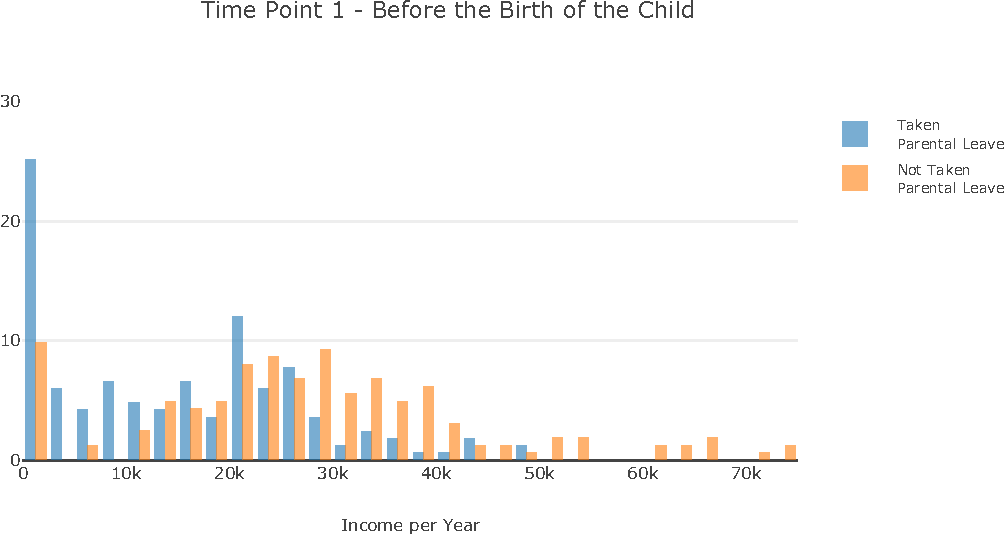
\includegraphics{Parental_Leave-GESS-VersionRmd_files/figure-latex/fig-1-1} 

}

\caption{Distribution of Income Between Persons Taking Parental Leave or not Before the Birth of the Child (Time Point 1)}\label{fig:fig-1}
\end{figure}

\begin{figure}

{\centering 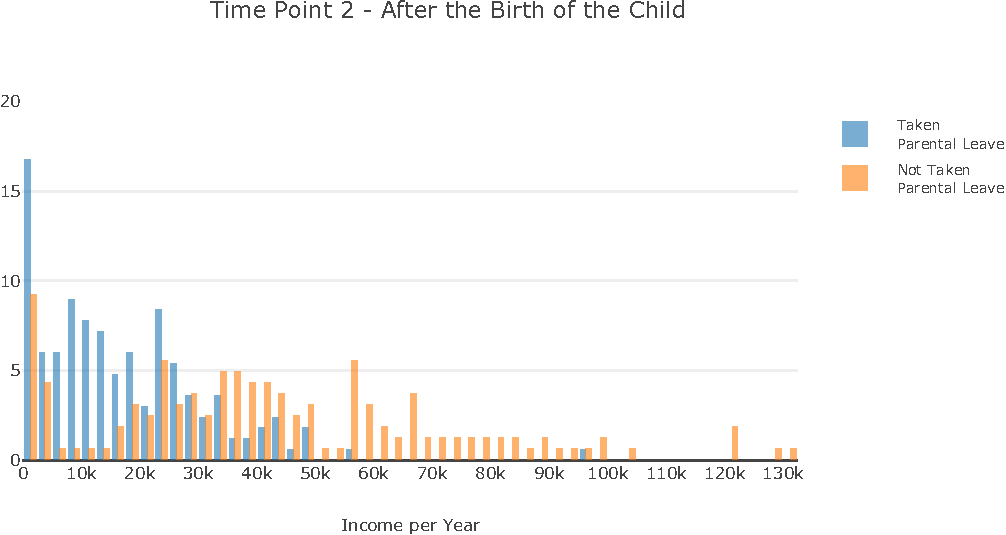
\includegraphics{Parental_Leave-GESS-VersionRmd_files/figure-latex/fig-2-1} 

}

\caption{Distribution of Income Between Persons Taking Parental Leave or not After the Birth of the Child (Time Point 2)}\label{fig:fig-2}
\end{figure}

\hypertarget{results}{%
\section{Results}\label{results}}

\hypertarget{influence-of-parental-leave}{%
\subsubsection*{\texorpdfstring{\emph{Influence of parental leave}}{Influence of parental leave}}\label{influence-of-parental-leave}}
\addcontentsline{toc}{subsubsection}{\emph{Influence of parental leave}}

The first hypothesis I proposed was referencing to the causal influence of taking parental leave on income in a long-term effect. In order to visualize the distribution of income at each time point I created a barplot shown in Figure \ref{fig:fig-1} \& \ref{fig:fig-2}. The x-axis describes the annual income for each individual and the y-axis shows the percentage.\footnote{Applies to all other graphs.} The color of the bars stand for the Individuals which took parental leave (blue) and for those who did not (orange). At time point 1, before the birth, both groups are centered around 20,000 to 30,000 euros per year. However the treatment group has more observations in the lower half and the control group is more represented in the higher income categories, indicating that there is some prior self selection.

The second barplot (figure \ref{fig:fig-2}) displays time point 2 (after birth) shows a distinct shift of both groups. The treatment group shifted towards the lower spectrum of income and the control group in the opposite direction, leaving a greater disparity between both groups. This implies that the parental leave might have an impact on income.

To further examine this assumption I run a linear regression on basis of a difference in differences model shown in table \ref{tab2}. M1 only tests the influence of taking parental leave on income. The results show, that if one is taking parental leave they are likely to earn 12,399.040 Euros less after 15 years compared to someone who did not take parental leave. These results are significant within a 99\% confidence interval. When introducing the control variables the coefficient of parental leave decreases and is now only significant within a 90\% confidence interval. Therefore, the hypothesis has to be rejected for a 0.05 alpha level.

\begin{table}[!htbp] \centering 
  \caption{Regression Table - Linear Regression on Basis of a Difference in Differences Model Testing for Hypothesis 1 and 3} 
  \label{tab2} 
\footnotesize 
\begin{tabular}{@{\extracolsep{-5pt}}lcccc} 
\\[-1.8ex]\hline 
\hline \\[-1.8ex] 
 & \multicolumn{4}{c}{\textit{Dependent variable:}} \\ 
\cline{2-5} 
\\[-1.8ex] & \multicolumn{4}{c}{Annual Income} \\ 
 & M1 & M2 & M3 & M4 \\ 
\hline \\[-1.8ex] 
 Parental Leave & $-$12,399.040$^{***}$ & $-$7,984.528$^{*}$ & $-$4,889.731 & $-$3,011.547 \\ 
  & (2,099.990) & (4,661.177) & (13,537.900) & (12,904.120) \\ 
  & & & & \\ 
 Male &  & $-$7,014.564 & $-$7,832.613 & $-$6,229.043 \\ 
  &  & (4,725.737) & (4,874.618) & (5,099.879) \\ 
  & & & & \\ 
 Age &  & 3,200.347 &  & 3,186.185 \\ 
  &  & (2,057.393) &  & (2,060.677) \\ 
  & & & & \\ 
 Age Squared &  & $-$57.642$^{*}$ &  & $-$57.503$^{*}$ \\ 
  &  & (30.259) &  & (30.305) \\ 
  & & & & \\ 
 West Germany &  & $-$963.382 &  & $-$1,026.475 \\ 
  &  & (2,637.065) &  & (2,645.316) \\ 
  & & & & \\ 
 Child Count &  & 1,014.902 &  & 1,029.209 \\ 
  &  & (1,251.661) &  & (1,253.963) \\ 
  & & & & \\ 
 High Education &  & 12,396.130$^{***}$ &  & 12,468.090$^{***}$ \\ 
  &  & (2,346.398) &  & (2,356.257) \\ 
  & & & & \\ 
 Occupation &  & $-$809.866$^{**}$ &  & $-$796.397$^{**}$ \\ 
  &  & (344.886) &  & (346.922) \\ 
  & & & & \\ 
 Parental Leave X Male &  &  & $-$599.617 & $-$5,732.633 \\ 
  &  &  & (14,378.260) & (13,867.910) \\ 
  & & & & \\ 
 Constant & 14,695.790$^{***}$ & $-$25,740.850 & 15,517.730$^{***}$ & $-$25,568.090 \\ 
  & (1,496.158) & (33,832.330) & (1,579.092) & (33,884.230) \\ 
  & & & & \\ 
\hline \\[-1.8ex] 
Observations & 329 & 294 & 329 & 294 \\ 
Adjusted R$^{2}$ & 0.094 & 0.200 & 0.096 & 0.198 \\ 
\hline 
\hline \\[-1.8ex] 
\textit{Note:}  & \multicolumn{4}{r}{$^{*}$p$<$0.1; $^{**}$p$<$0.05; $^{***}$p$<$0.01} \\ 
\end{tabular} 
\end{table}

\hypertarget{length-of-parental-leave}{%
\subsubsection*{\texorpdfstring{\emph{Length of Parental Leave}}{Length of Parental Leave}}\label{length-of-parental-leave}}
\addcontentsline{toc}{subsubsection}{\emph{Length of Parental Leave}}

** Parts (Graph Hypothesis 2) excluded due to Word Limit **

The second hypothesis proposed the idea, that the length of parental leave influences income. This assumption seems to hold true according to Model 1 (M1) of Table \ref{tab3} which displays only the influence of the length of the parental leave on the income difference. By taking a longer parental leave, the income after 15 years will be about 6,486,803 higher than for a person who has taken only a short leave. This result is significant within a 90 \% confidence interval. However, as the results are not conform with the hypothesis which were proposed, hypothesis 2 has to be rejected.

\begin{table}[!htbp] \centering 
  \caption{Regression Table - Linear Regression on Basis of a Difference in Differences Model Testing for Hypothesis 2} 
  \label{tab3} 
\footnotesize 
\begin{tabular}{@{\extracolsep{-5pt}}lcc} 
\\[-1.8ex]\hline 
\hline \\[-1.8ex] 
 & \multicolumn{2}{c}{\textit{Dependent variable:}} \\ 
\cline{2-3} 
\\[-1.8ex] & \multicolumn{2}{c}{Annual Income} \\ 
 & M1 & M2 \\ 
\hline \\[-1.8ex] 
 Long Leave & 6,486.803$^{*}$ & 6,016.711$^{*}$ \\ 
  & (3,624.890) & (3,341.767) \\ 
  & & \\ 
 Female &  & $-$11,455.770 \\ 
  &  & (9,967.716) \\ 
  & & \\ 
 Age &  & 9,003.787$^{***}$ \\ 
  &  & (3,030.618) \\ 
  & & \\ 
 Age Squared &  & $-$152.280$^{***}$ \\ 
  &  & (48.250) \\ 
  & & \\ 
 West Germany &  & $-$8,630.072$^{***}$ \\ 
  &  & (2,796.995) \\ 
  & & \\ 
 Child Count &  & 5,462.574$^{***}$ \\ 
  &  & (1,424.138) \\ 
  & & \\ 
 High Education &  & 4,167.398 \\ 
  &  & (2,673.758) \\ 
  & & \\ 
 Occupation &  & $-$813.028$^{**}$ \\ 
  &  & (335.953) \\ 
  & & \\ 
 Constant & $-$3,335.500 & $-$116,962.800$^{**}$ \\ 
  & (3,377.696) & (48,306.780) \\ 
  & & \\ 
\hline \\[-1.8ex] 
Observations & 167 & 153 \\ 
Adjusted R$^{2}$ & 0.013 & 0.251 \\ 
\hline 
\hline \\[-1.8ex] 
\textit{Note:}  & \multicolumn{2}{r}{$^{*}$p$<$0.1; $^{**}$p$<$0.05; $^{***}$p$<$0.01} \\ 
\end{tabular} 
\end{table}

\hypertarget{interaction-effect-between-parental-leave-and-gender}{%
\subsubsection*{\texorpdfstring{\emph{Interaction effect between Parental Leave and Gender}}{Interaction effect between Parental Leave and Gender}}\label{interaction-effect-between-parental-leave-and-gender}}
\addcontentsline{toc}{subsubsection}{\emph{Interaction effect between Parental Leave and Gender}}

** Parts (Graph Hypothesis 3) excluded due to Word Limit **

To test the third hypothesis, which states that women who take parental leave have a larger decline in earnings, I run two regressions. First, only the interaction between gender and parental leave is displayed in Table \ref{tab2} model 3 (M3). None of the coefficients in this model are significant. The same applies to model 4. This suggests that adding the interaction has an effect on the long term effect of parental leave. As there were no significant results found, the third hypothesis has to be rejected.

\hypertarget{conclusion-and-discussion}{%
\section{Conclusion and Discussion}\label{conclusion-and-discussion}}

\hypertarget{conclusion}{%
\subsubsection*{\texorpdfstring{\emph{Conclusion}}{Conclusion}}\label{conclusion}}
\addcontentsline{toc}{subsubsection}{\emph{Conclusion}}

The results give contradictory implications in regard to answering the research question whether parental leave has a negative impact on future income or not. On the one hand the results regarding hypothesis 1 are in line with prior research (Evertsson \protect\hyperlink{ref-evertsson_parental_2016}{2016}; Stafford and Sundström \protect\hyperlink{ref-stafford_time_1996}{1996}). There is (small) significant evidence that parental leave has a negative impact on future income. Presumably due to missed opportunities at work and the resulting decline in human capital, leading to long lasting effects in the work field.

On the other hand, contrary to the human capital theory, there are significant results showing that a long parental leave has positive effects on the future income compared to a short leave, contrary to my former hypothesis.
These results might be explained by the signaling theory. Contrary to the belief of many scholars, that parental leave would signal less commitment to the company and might imply a low work ethic, this might only be true for the general impact of parental leave (Albrecht et al. \protect\hyperlink{ref-albrecht_career_1999}{1999}; Evertsson \protect\hyperlink{ref-evertsson_parental_2016}{2016}; Stafford and Sundström \protect\hyperlink{ref-stafford_time_1996}{1996}). However, a long parental leave could be also a signal for other characteristics which might be more important. When someone stays longer in parental leave, they show dedication, as they leave their job to sacrifice their career to care for their child, especially when staying for a longer period. Additionally, it implies openness and adaptability as carrying for a newborn is a challenging task and demand constant adaption to new situations.
Furthermore, I did not find significant results to substantiate my third hypothesis. These results might be due to the small number of observations, especially in male parental leave groups. Additionally, in today's time more men are taking parental leave, compared to the 1990s. So it is hard to make a valid statement on basis of these results.

\hypertarget{limitations}{%
\subsubsection*{\texorpdfstring{\emph{Limitations}}{Limitations}}\label{limitations}}
\addcontentsline{toc}{subsubsection}{\emph{Limitations}}

Despite everything, there are some major shortcomings to this study. First and foremost, the number of observations is really small.
Which leads to a discrimination with respect to certain characteristics. Also because of this, I was not able to do a matching process which may have helped to control for self-selection. Especially in Figure \ref{fig:fig-1} (t1), we can notice a severe difference between the control and treatment group, suggesting that there was happening some sort of self-selection. This is especially noticeable for males which took parental leave. There are only a few in this data set.

** Parts Excluded due to word limit **

Another problem is the large number of people who started with no income. Due to the study design, if later a job is found, the income is counted as increase.\\
However, I tried to counterbalance that as I only included persons which were 21 or older, so the probability that they have a job is much higher.

And lastly, even though I dropped all cases where someone had more than one child during the observation time period. There might been women who did more than one parental leave, however, as the variable was not featured in every wave, I could not control for that either.

\hypertarget{future-research}{%
\subsubsection*{\texorpdfstring{\emph{Future Research}}{Future Research}}\label{future-research}}
\addcontentsline{toc}{subsubsection}{\emph{Future Research}}

** Parts Excluded due to word limit **

\hypertarget{statutory-declaration}{%
\section*{Statutory Declaration}\label{statutory-declaration}}
\addcontentsline{toc}{section}{Statutory Declaration}

I hereby declare that the paper presented is my own work and that I have not called upon the help of a third party. In addition, I affirm that neither I nor anybody else has submitted this paper or parts of it to obtain credits elsewhere before. I have clearly marked and acknowledged all quotations or references that have been taken from the works of other. All secondary literature and other sources are marked and listed in the bibliography. The same applies to all charts, diagrams and illustrations as well as to all Internet sources. Moreover, I consent to my paper being electronically stores and sent anonymously in order to be checked for plagiarism. I am aware that the paper cannot be evaluated and may be graded ``failed'' (``nicht ausreichend'') if the declaration is not made.

Place, Date: Mannheim, 15.07.2020

Signature:
(Sophie Hensgen)

\newpage

\hypertarget{bibliography}{%
\section*{Bibliography}\label{bibliography}}
\addcontentsline{toc}{section}{Bibliography}

\hypertarget{refs}{}
\leavevmode\hypertarget{ref-albrecht_career_1999}{}%
Albrecht, James W., Per-Anders Edin, Marianne Sundstrom, and Susan B. Vroman. 1999. ``Career Interruptions and Subsequent Earnings: A Reexamination Using Swedish Data.'' \emph{The Journal of Human Resources} 34(2):294.

\leavevmode\hypertarget{ref-becker_human_1993}{}%
Becker, Gary S. 1993. \emph{Human Capital: A Theoretical and Empirical Analysis, with Special Reference to Education}. 3rd ed. Chicago: The University of Chicago Press.

\leavevmode\hypertarget{ref-dribe_does_2009}{}%
Dribe, Martin and Maria Stanfors. 2009. ``Does Parenthood Strengthen a Traditional Household Division of Labor? Evidence from Sweden.'' \emph{Journal of Marriage and Family} 71(1):33--45.

\leavevmode\hypertarget{ref-evertsson_parental_2016}{}%
Evertsson, Marie. 2016. ``Parental Leave and Careers: Women's and Men's Wages After Parental Leave in Sweden.'' \emph{Advances in Life Course Research} 29:26--40.

\leavevmode\hypertarget{ref-gabriele_mari_parental_2019}{}%
Gabriele Mari and Giorgio Cutuli. 2019. ``Do Parental Leaves Make the Motherhood Wage Penalty Worse? Assessing Two Decades of German Reforms.'' \emph{Deutsches Institut F\textbackslash"\{u\}r Wirtschaftsforschung (DIW)} 1025:http://hdl.handle.net/10419/194106.

\leavevmode\hypertarget{ref-geisler_against_2011}{}%
Geisler, Esther and Michaela Kreyenfeld. 2011. ``Against All Odds: Fathers' Use of Parental Leave in Germany.'' \emph{Journal of European Social Policy} 21(1):88--99.

\leavevmode\hypertarget{ref-grabka_soep_2017}{}%
Grabka, Markus M. 2017. ``SOEP 2016 -- Codebook for the \$PEQUIV File 1984-2016: CNEF Variables with Extended Income Information for the SOEP.''

\leavevmode\hypertarget{ref-helen_dearing_does_2015}{}%
Helen Dearing. 2015. ``Does Parental Leave Influence the Gender Dividon of Labour? Recent Empirical Findings from Europe.''

\leavevmode\hypertarget{ref-hofferth_parental_2006}{}%
Hofferth, Sandra L. and Sally C. Curtin. 2006. ``Parental Leave Statutes and Maternal Return to Work After Childbirth in the United States.'' \emph{Work and Occupations} 33(1):73--105.

\leavevmode\hypertarget{ref-lapuerta_individual_2011}{}%
Lapuerta, Irene, Pau Baizán, and María José González. 2011. ``Individual and Institutional Constraints: An Analysis of Parental Leave Use and Duration in Spain.'' \emph{Population Research and Policy Review} 30(2):185--210.

\leavevmode\hypertarget{ref-liebig_socio-economic_2019}{}%
Liebig, Stefan, Jan Goebel, Carsten Schröder, Markus Grabka, David Richter, Jürgen Schupp, Charlotte Bartels, Alexandra Fedorets, Andreas Franken, Jannes Jacobsen, Selin Kara, Peter Krause, Hannes Kröger, Martin Kroh, Maria Metzing, Jana Nebelin, Diana Schacht, Paul Schmelzer, Christian Schmitt, Daniel Schnitzlein, Rainer Siegers, Knut Wenzig, Stefan Zimmermann, and Deutsches Institut Für Wirtschaftsforschung (DIW Berlin). 2019. ``Socio-Economic Panel (SOEP), Data from 1984-2018Sozio-Oekonomisches Panel (SOEP), Daten Der Jahre 1984-2018.''

\leavevmode\hypertarget{ref-marshall_fathers_2008}{}%
Marshall, Katherine. 2008. ``Father's Use of Paid Parental Leave.'' \emph{Perspectives on Labour and Income} 9.

\leavevmode\hypertarget{ref-mignot_peter_2011}{}%
Mignot, J.-F. and G. Manzo. 2011. ``Peter Hedstrom and Peter Bearman (Eds.): The Oxford Handbook of Analytical Sociology.'' \emph{European Sociological Review} 27(6):824--35.

\leavevmode\hypertarget{ref-misra_work-family_2011}{}%
Misra, Joya, Michelle Budig, and Irene Boeckmann. 2011. ``Work-Family Policies and the Effects of Children on Women's Employment Hours and Wages.'' \emph{Community, Work \& Family} 14(2):139--57.

\leavevmode\hypertarget{ref-plantenga_reconciliation_2005}{}%
Plantenga, J. and Chantal. Remery. 2005. \emph{Reconciliation of Work and Private Life: A Comparative Review of Thirty European Countries.}

\leavevmode\hypertarget{ref-pronzato_return_2009}{}%
Pronzato, Chiara Daniela. 2009. ``Return to Work After Childbirth: Does Parental Leave Matter in Europe?'' \emph{Review of Economics of the Household} 7(4):341--60.

\leavevmode\hypertarget{ref-ridgeway_unpacking_2004}{}%
Ridgeway, Cecilia L. and Shelley J. Correll. 2004. ``Unpacking the Gender System: A Theoretical Perspective on Gender Beliefs and Social Relations.'' \emph{Gender \& Society} 18(4):510--31.

\leavevmode\hypertarget{ref-rostgaard_parental_2020}{}%
Rostgaard, Tine, Mogens Christoffersen, and Hanne Weise. 2020. ``Parental Leave in Denmark.''

\leavevmode\hypertarget{ref-stafford_time_1996}{}%
Stafford, Frank P. and Marianne Sundström. 1996. ``Time Out for Childcare: Signalling and Earnings Rebound Effects for Men and Women.'' \emph{Labour} 10(3):609--29.

\leavevmode\hypertarget{ref-statistisches_bundesamt_zeitreihe_2020}{}%
Statistisches Bundesamt. 2020. ``Zeitreihe: Entwicklung Des Väteranteils Nach Ländern. Destatis- Statistisches Bundesamt.''

\end{document}
